\documentclass{beamer}

\mode<presentation>
{
\usetheme{Madrid}
}

\usepackage{graphics, graphicx}
\usepackage{booktabs}
\DeclareGraphicsExtensions{.pdf,.png,.jpg,.gif}

\title{Linux Beginner Guide}

\author{Jaewoong Lee}

\institute[UNIST]
{
	Ulsan National Institute of Science and Technology
	\medskip
	\newline
	\textit{jwlee230@unist.ac.kr}
}

\date{\today}

\begin{document}
	\begin{frame}
		\titlepage
	\end{frame}

	\begin{frame}
		\frametitle{Introduction}
		
		In this guide, I assume that followings are already installed:
		\begin{enumerate}
			\item Ubuntu 16.04.2 or Higher
			\item ZSH 5.0.2 or Higher
			\item VIM 8.1 or Higher
		\end{enumerate}

		With this guide, you can use and understand Linux system. \\
		Also, this guide includes as little information about operating system as possible. If you find some fault in the strict sense of the word, that means you are not \textbf{beginner}. 
	\end{frame}

	\begin{frame}
		\frametitle{Overview}
		\tableofcontents
	\end{frame}

	\section{Linux?}
	
	\begin{frame}
		\frametitle{Linux?}
		\begin{figure}[h!]
			\centering
			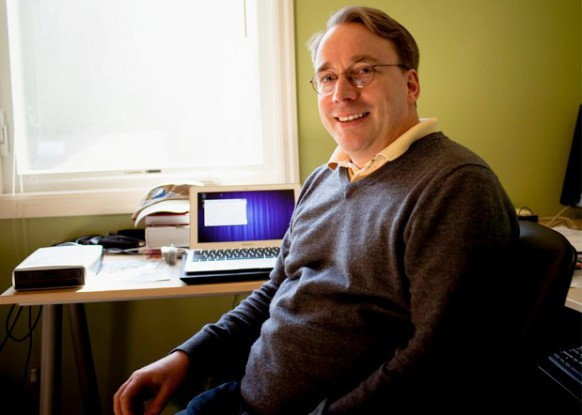
\includegraphics[width=0.3 \linewidth]{figures/linus.jpg}
			\caption{Linus Torvalds, Inventor of Linux}
		\end{figure}
	
		Linux is one of the most famous OS as Windows and macOS. 
	\end{frame}
	
	\section{Basic Linux Command}
	
	\section{Edit File with VIM}
	
	\section{How to Download from Web}
	
	\section{User Permissions}
	
	\section{IO Redirections}
	
	\section{Process Control}
	
	\section{Process Control with SGE}

\end{document}